\documentclass[10pt, conference]{IEEEtran/IEEEtran}

\usepackage{graphicx}
\usepackage{color}
\usepackage{amsmath}
\usepackage{float}
\usepackage[all]{xy}
\usepackage[font=small]{caption}
\usepackage{hyperref}


\begin{document}

\title{Performance Analysis of TCP Variants}

\author{\IEEEauthorblockN{Liang Tian}
\IEEEauthorblockA{College of Computer and Information Science\\
Northeastern University, MA, 02115\\
Email: ltian@ccs.neu.edu\\}
\and
\IEEEauthorblockN{Yang Cai}
\IEEEauthorblockA{College of Computer and Information Science\\
Northeastern University, MA, 02115\\
Email: yang@ccs.neu.edu\\}
}
\maketitle
\begin{abstract}
In this paper we conduct simulation-based experiments to analyze performance of  TCP variants Tahoe, Reno, New Reno and Vegas, in particular their performances against congestion, as well as fairness between TCP variants for pairs Reno/Reno, New Reno/Reno, Vegas/Vegas, New Reno/Vegas. In addition, we analyze the influence of choice of queueing algorithms for Reno and SACK TCP.
\end{abstract}
\section{Introduction}
There are many TCP variants and many of them are implemented in some systems. In this paper we simulate Tahoe, Reno, New Reno and Vegas, compare their performances under congestion, as well as when they co-exit with other TCP variants (as in the real world). Also we explore the benefits of introducing SACK (selective acknowledgements)  and how well SACK works with RED and DropTail queueing disciplines.

As a quick review, we highlight some features we are interested in for each of the TCP variant\cite{sim}:

TCP Tahoe: \textit{Fast Retransmit}, after receiving a small number of duplicate acknowledgements for the same TCP segments (dup ACKs), the data sender infers that a packet has been lost and retransmits the packet without waiting for a retransmission timer to expire, leading to higher channel utilization and connection throughput.

TCP Reno: \textit{Fast Recovery}, prevents the communication path from going empty after Fast Retransmit, thereby avoiding the need to Slow-Start to re-fill it after a packet loss.

TCP New Reno: The New-Reno TCP in this paper includes a small change to the Reno algorithm at the sender that eliminates Reno's wait for a retransmit timer when multiple packets are lost from a window. \cite{sim}

Vegas TCP: TCP Vegas is a TCP congestion avoidance algorithm that emphasizes packet delay, rather than packet loss, as a signal to help determine the rate at which to send packets. TCP Vegas detects congestion at an incipient stage based on increasing Round-Trip Time (RTT) values of the packets in the connection unlike other flavors such as Reno, New Reno, etc., which detect congestion only after it has actually happened via packet loss. The algorithm depends heavily on accurate calculation of the Base RTT value. If it is too small then throughput of the connection will be less than the bandwidth available while if the value is too large then it will overrun the connection.
%
%A lot of research is going on regarding the fairness provided by the linear increase/decrease mechanism for congestion control in Vegas. 


\section{Methodology}

We use simulator \textit{ns2} which runs the experiment with given configuration specified in a tcl file, and
  output a trace file that we can analyze packets transmission. All computations and plots are done with Python.

We want to compare performances of TCP variants in the following scenarios: under congestion, co-existing with other variants under congestion, working with different queueing algorithms implemented at the gateways. The details specifications are given in each experiment in next section.
\subsection*{Notations}

We define throughput, latency, drop-rate as follows:

\[
\text{throughput}= \frac{\text{\# of received packets} \cdot \text{packet size}}{\text{duration of connection}}
\]
where we count the number of received unique ACKs at the sender agent and use it as \textbf{number of received packets}. Here ACKs must be unique because they could be duplicated, which means that there are packet losses.
\[
\text{latency}=\frac{\text{sum of RTT of all received packets} }{\text{\# of packets received}}
\]
where RTT is Round-Trip Time: we record the time it takes from a packet is enqueued at the sender agent(denoted as "+" in NS2 trace file) till the first ACK for the packet is received at the sender agent.
\[
\text{drop-rate}: \frac{\text{(\# sent packets - \# received packets)}}{\text{\# sent packets}}
\]
\section{Experiments}
In all experiments below, we use the same simple network topology as shown in the following graph:

\centerline{
\xymatrix{
N1 \ar@{-}[dr] & & & N4\\
& N2\ar@{-}[r]  & N3\ar@{-}[dr] \ar@{-}[ur]  & \\
N5\ar@{-}[ur]  &  &  & N6\\
}
}

\subsection{Experiment 1: TCP Performance Under Congestion}
\subsubsection{Configuration}

In this experiment, we want to explore performance of TCP variants under Congestion. So in each simulation, we set up a CBR source at N2 and sink at N3, between which there is a UDP data stream. One single TCP stream from N1 to N4 is introduced a few seconds after simulation starts.

To simulate different congestion levels, we vary CBR from 0.5 to 10 Mbps for each TCP variants Tahoe, Reno, New Reno and Vegas.


\subsubsection{Results Analysis}

\begin{figure}[!ht]
\begin{center}
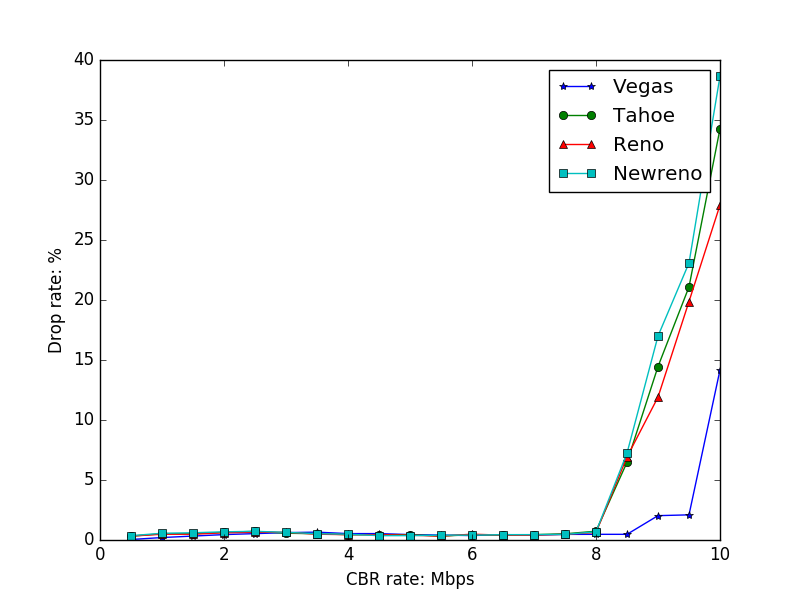
\includegraphics[width=\linewidth]{../exp1/exp1_drop.png}
\caption{Drop rate of TCP variants under different CBR rates}
\label{exp1_drop}
\end{center}
\end{figure}

\begin{figure}[!ht]
\begin{center}
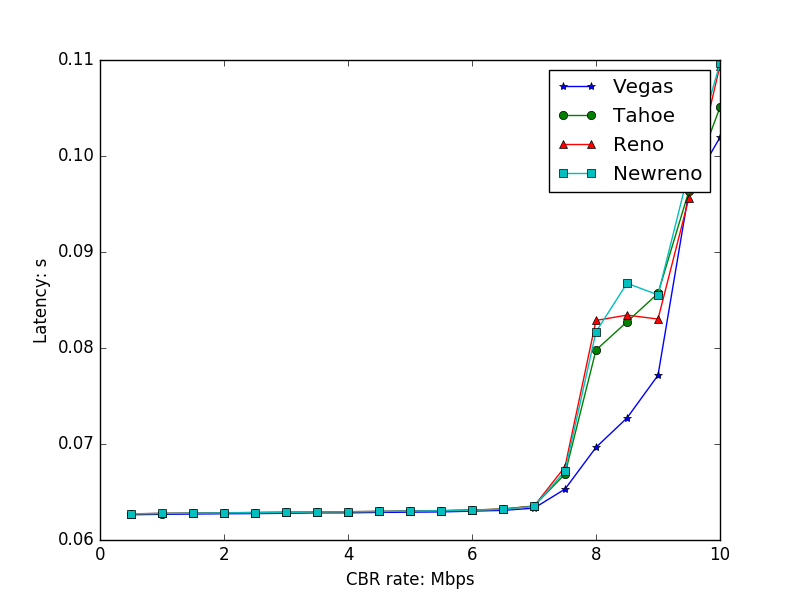
\includegraphics[width=\linewidth]{../exp1/exp1_lat.png}
\caption{Latency of TCP variants under different CBR rates}
\label{exp1_lat}
\end{center}
\end{figure}

\begin{figure}[!ht]
\begin{center}
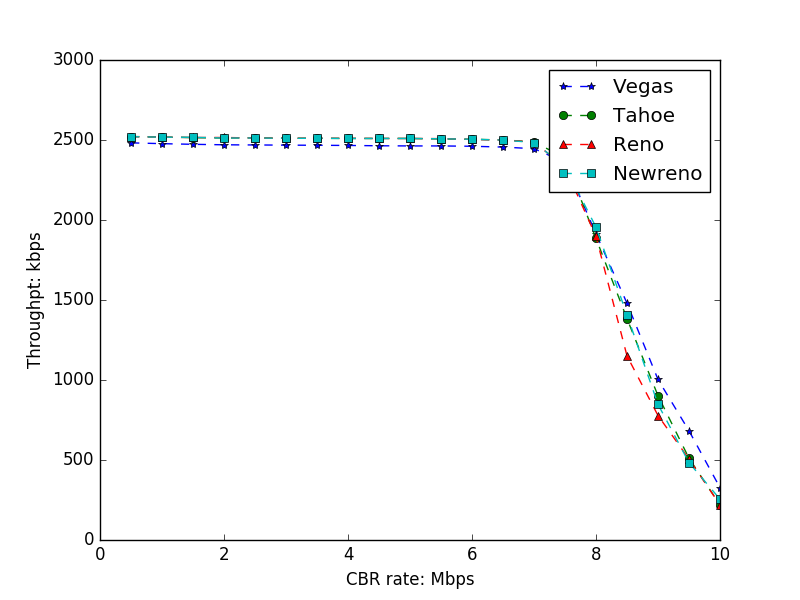
\includegraphics[width=\linewidth]{../exp1/exp1_thpt.png}
\caption{Throughput of TCP variants under different CBR rates}
\label{exp1_thpt}
\end{center}
\end{figure}

Fig. \ref{exp1_drop}, Fig. \ref{exp1_lat} and Fig. \ref{exp1_thpt} show the drop-rate, average latency and throughput for each TCP variant when the CBR rate varies from 0.5 to 10Mbps. 

We can see that when CBR rate is lower than 7Mbps, all TCP variants performs almost the same except Vegas has slightly lower throughput. When congestion becomes more and more severe, TCP Vegas starts to stand out while all others remain having similar performance. TCP Vegas has significantly lower drop-rate and level of latency and throughput is higher. So overall, TCP Vegas is better except that even when congestion level is low it already slows down slightly as it can detect congestion earlier than others\cite{vegas}.

To show that this is a statistically significant result, (i.e., it is the different implementations of TCP variants that is causing the difference in their average latency and drop-rate, instead of other parameters and random noise,) we run the simulation for each CBR rate for 10 times, each time we simulate with different values for the parameters

\begin{itemize}
\item start time of the TCP stream
\item packet size
\end{itemize}

\textbf{t-test}
An interesting fact is that for CBR between 8 and 9.5Mbps, latency of Tahoe/Reno/NewReno don't change that much compared to when CBR changes from 7.5 to 8Mbps.
An interesting fact is that for CBR between 8 and 9.5Mbps, latency of Tahoe/Reno/NewReno don't change that much compared to when CBR changes from 7.5 to 8Mbps.
An interesting fact is that for CBR between 8 and 9.5Mbps, latency of Tahoe/Reno/NewReno don't change that much compared to when CBR changes from 7.5 to 8Mbps.
An interesting fact is that for CBR between 8 and 9.5Mbps, latency of Tahoe/Reno/NewReno don't change that much compared to when CBR changes from 7.5 to 8Mbps.

An interesting fact is that for CBR between 8 and 9.5Mbps, latency of Tahoe/Reno/NewReno don't change that much compared to when CBR changes from 7.5 to 8Mbps.

\subsection{Experiment 2: Fairness Between TCP Variants}

In this experiment, we want to analyze fairness between TCP variants. To do so, we set up a CBR source at N2 and sink at N3 and a UDP stream between them. We start one TCP stream from N1 to N4 using one TCP
variant and another TCP stream from N5 to N6 using another TCP variant.

As in previous experiment, the configuration of the simulation iterate over the combinations of 
\begin{itemize}
\item Each pair of TCP variants(one of Reno/Reno, New Reno/Reno, Vegas/Vegas,
New Reno/Vegas), 
\item CBR from 0.5 to 10Mbps.
\end{itemize}

%Reno/Reno
\subsubsection{Reno/Reno}
\begin{figure}[!ht]
\begin{center}
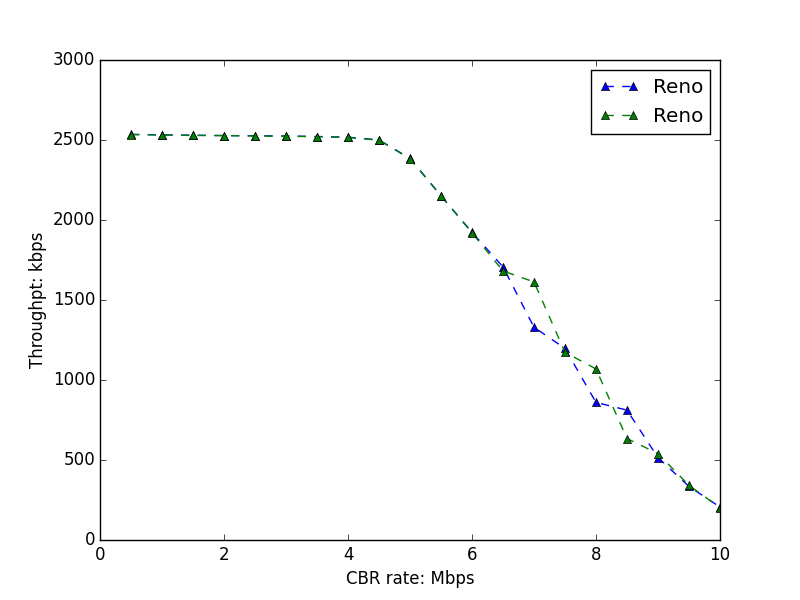
\includegraphics[width=\linewidth]{../exp2/exp2_Reno_Reno_thpt.png}
\caption{Throughput of Reno/Reno under different CBR rates}
\label{exp2_Reno_Reno_thpt}
\end{center}
\end{figure}

By comparing the drop-rate , throughput and latency of the two TCP streams,  we can see that their performances are very similar, so Reno is fair to itself. 
Fig.\ref{exp2_Reno_Reno_thpt} shows throughputs of the two TCP Reno streams.

%New Reno/Reno
\subsubsection{New Reno/Reno}
\begin{figure}[!ht]
\begin{center}
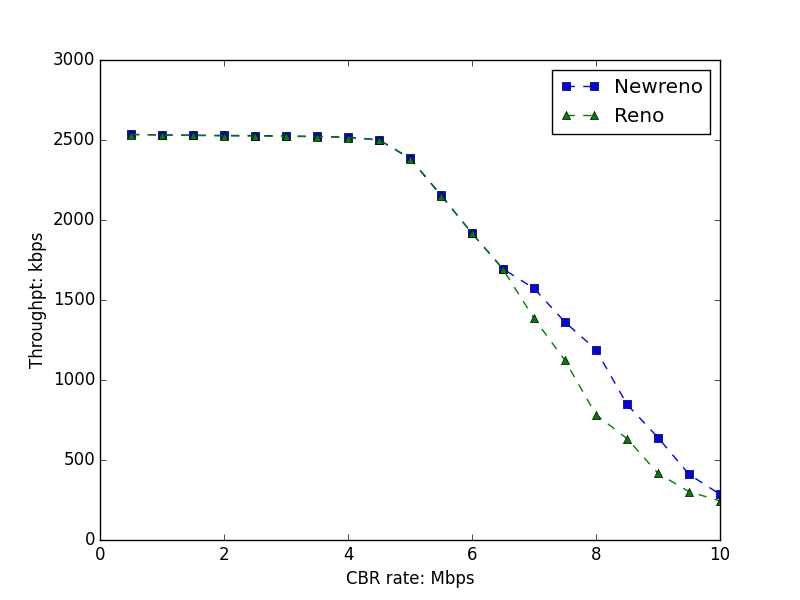
\includegraphics[width=\linewidth]{../exp2/exp2_Newreno_Reno_thpt.png}
\caption{Throughput of NewReno/Reno under different CBR rates}
\label{exp2_NewReno_Reno_thpt}
\end{center}
\end{figure}
\begin{figure}[!ht]
\begin{center}
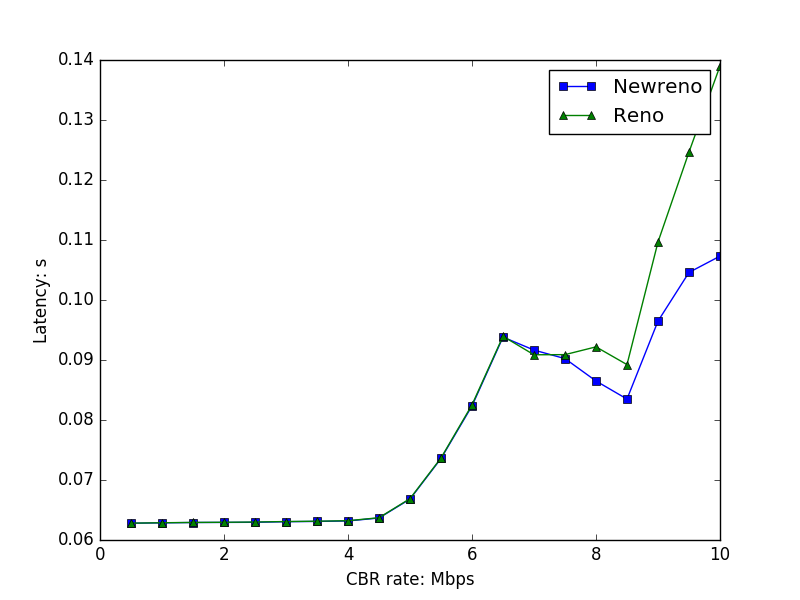
\includegraphics[width=\linewidth]{../exp2/exp2_Newreno_Reno_lat.png}
\caption{Latency of NewReno/Reno under different CBR rates}
\label{exp2_NewReno_Reno_lat}
\end{center}
\end{figure}
%Why?
Fig.\ref{exp2_NewReno_Reno_thpt} and Fig.\ref{exp2_NewReno_Reno_lat} shows throughput and latency of the two TCP NewReno streams. 

It's clear that New Reno is not fair to Reno. New Reno is getting more throughput and maintains lower latency when congestion level gets high. The reason for this is that, as stated in previous section and \cite{sim}, New Reno eliminates Reno's wait for a retransmit timer when multiple packets are lost from a window. So when multiple packets are lost, Reno will wait for a timeout before try to retransmit but New Reno will retransmit immediately, which helps New Reno to get lower latency and transmit more throughput.



\subsubsection{Vegas/Vegas}
% only 1 figure here.
\begin{figure}[!hb]
\begin{center}
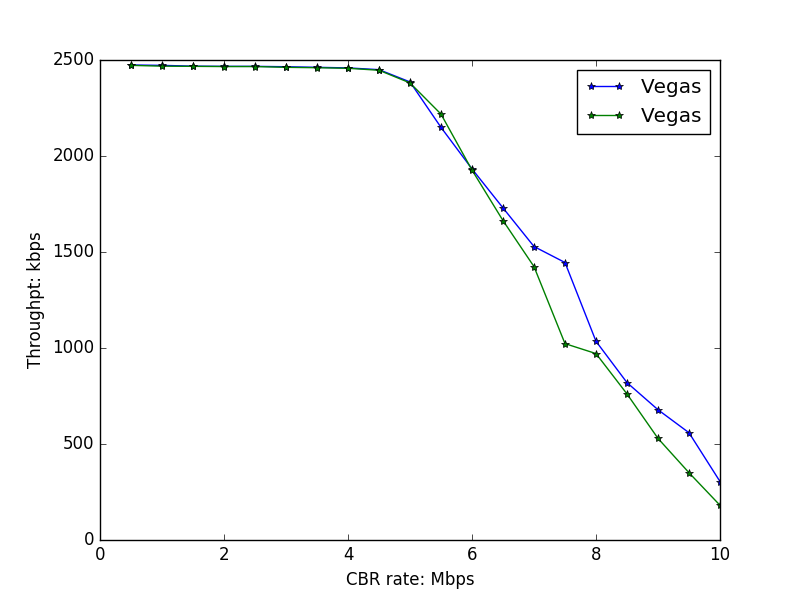
\includegraphics[width=\linewidth]{../exp2/exp2_Vegas_Vegas_thpt.png}
\caption{Throughput of Vegas/Vegas under different CBR rates}
\label{exp2_Vegas_Vegas_thpt}
\end{center}
\end{figure}
This case is similar to what we saw with Reno/Reno, Vegas is fair to itself, as shown in Fig.\ref{exp2_Vegas_Vegas_thpt}.
%New Reno/Vegas
\subsubsection{New Reno/Vegas}


Performance of Vegas degrades because Vegas reduces its sending rate before New Reno, as it detects congestion early and hence gives greater bandwidth to co-existing TCP Reno flows.
\begin{figure}[!h]
\begin{center}
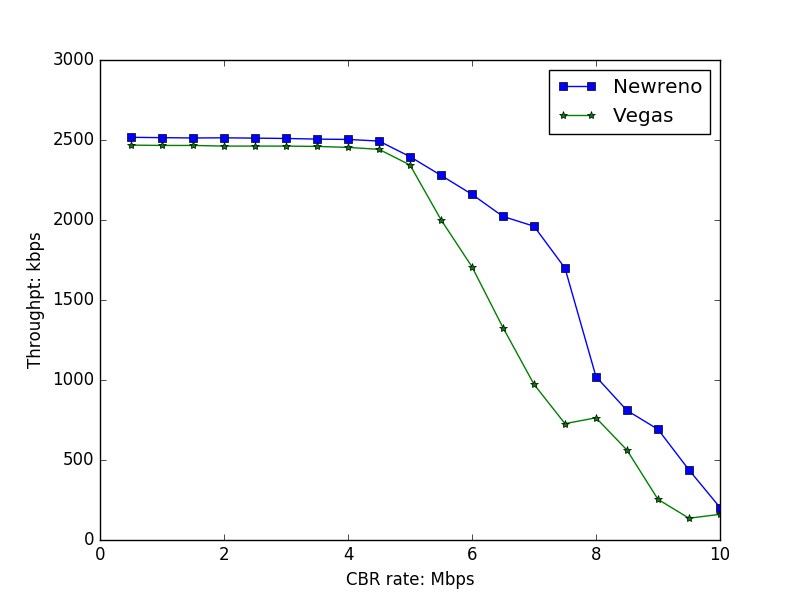
\includegraphics[width=\linewidth]{../exp2/exp2_Newreno_Vegas_thpt.png}
\caption{Throughput of New Reno/Vegas under different CBR rates}
\label{exp2_NewReno_Vegas_thpt}
\end{center}
\end{figure}




\subsection{Experiment 3: Influence of Queuing}

\subsubsection{Configuration}

For each queueing algorithm DropTail and RED:

Use TCP Reno and SACK to create two TCP flows N1 to N4 and N5 to N6, after 5 
seconds, introduce CBR from N2 to N3. Repeat the experiment for different CBR 
bandwidths.

\subsubsection{Results Analysis}

\begin{figure}[htbp]
\begin{center}
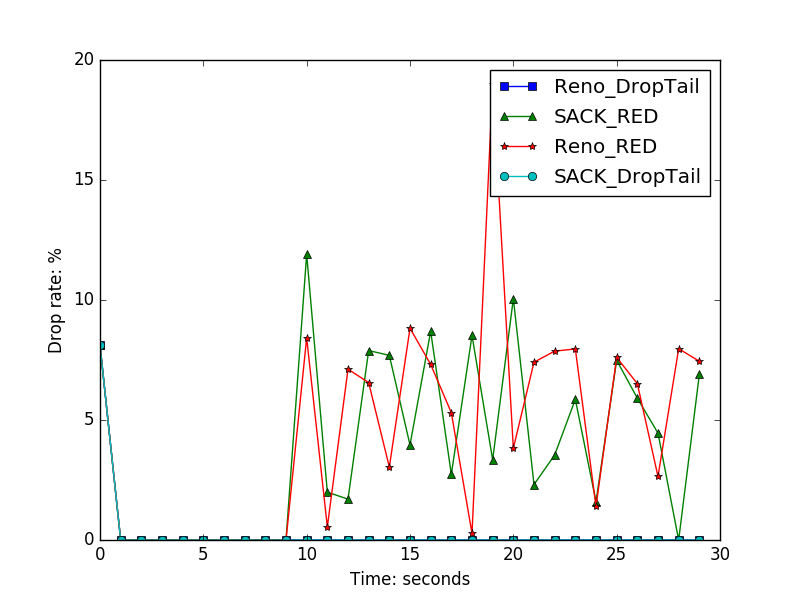
\includegraphics[width=\linewidth]{../exp3/exp3_drop.png}
\caption{Drop rate of TCP variants with different queueing algorithm}
\label{exp3_drop}
\end{center}
\end{figure}

\begin{figure}[htbp]
\begin{center}
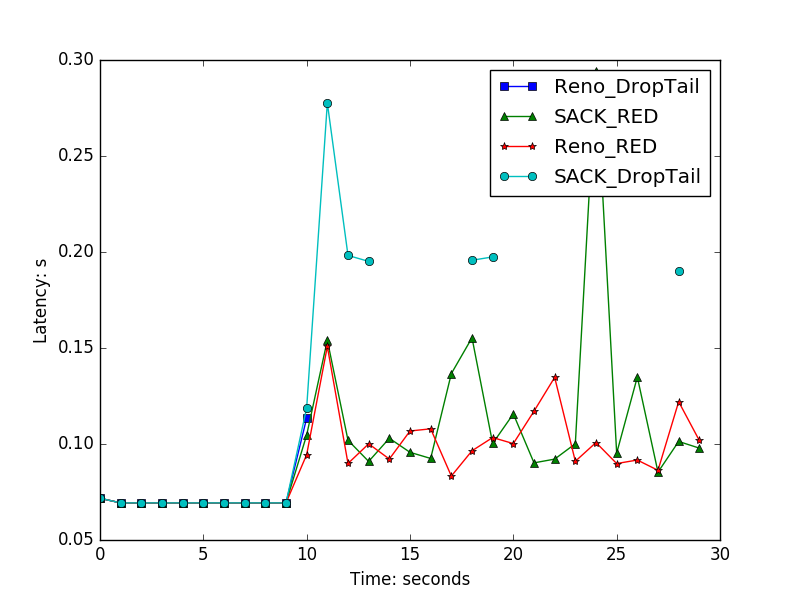
\includegraphics[width=\linewidth]{../exp3/exp3_lat.png}
\caption{Latency of TCP variants with different queueing algorithm}
\label{exp3_lat}
\end{center}
\end{figure}

\begin{figure}[htbp]
\begin{center}
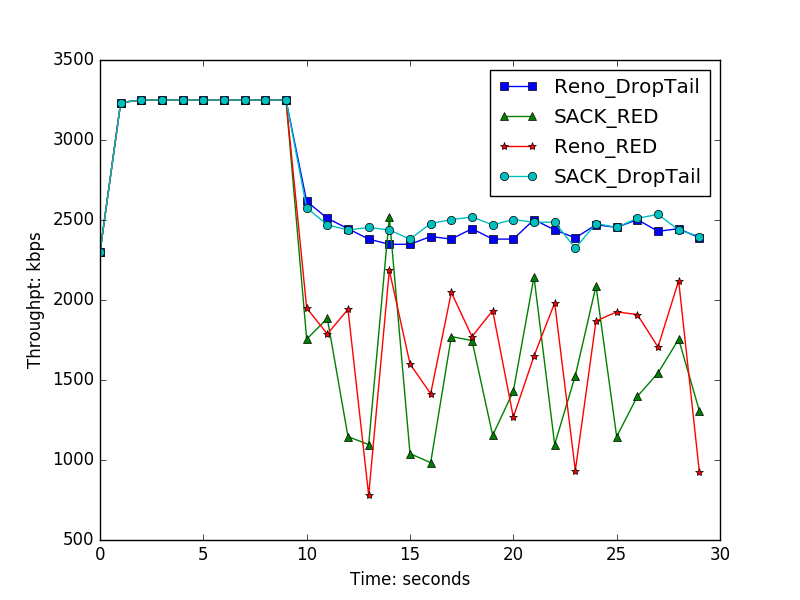
\includegraphics[width=\linewidth]{../exp3/exp3_thpt.png}
\caption{Throughput of TCP variants with different queueing algorithm}
\label{exp3_thpt}
\end{center}
\end{figure}
\section{Conclusion}

\begin{thebibliography}{50}
\bibitem{sim} Fall, Kevin, and Sally Floyd. ``Simulation-based comparisons of Tahoe, Reno and SACK TCP.''\textit{ACM SIGCOMM Computer Communication Review}
 26.3 (1996): 5-21.
 \bibitem{vegas}  \url{https://en.wikipedia.org/wiki/TCP_Vegas}
 \bibitem{vegas_red} Weigle, Eric, and Wu-chun Feng. ``A case for TCP Vegas in high-performance computational grids.'' 
 \textit{High Performance Distributed Computing, 2001. Proceedings. 10th IEEE International Symposium on}. IEEE, 2001. \bibitem{sim} Fall, Kevin, and Sally Floyd. "Simulation-based comparisons of Tahoe, Reno and SACK TCP." \textit{ACM SIGCOMM Computer Communication Review}
 26.3 (1996): 5-21.

\end{thebibliography}



\end{document}
